\documentclass[12pt,a4paper]{article}
\usepackage[margin=15mm,bottom=30mm,footskip=15mm]{geometry}
\usepackage{multicol}
\usepackage{graphicx}
\usepackage{titlesec}
\usepackage{cite}
\usepackage{caption}
\usepackage{subcaption}
\usepackage{hyperref}
\usepackage{float}

\titleformat{\section}{\Large\scshape\centering}{\romannumeral\thesection.}{3mm}{}
\setlength{\columnsep}{6mm}
\setlength{\belowcaptionskip}{-10pt}
\renewcommand{\thesubfigure}{\arabic{subfigure}}
\hypersetup{colorlinks=true}

\begin{document}
    \begin{titlepage}
        \centering

        \vspace*{2cm}
        \begin{figure}[h]
            \centering
            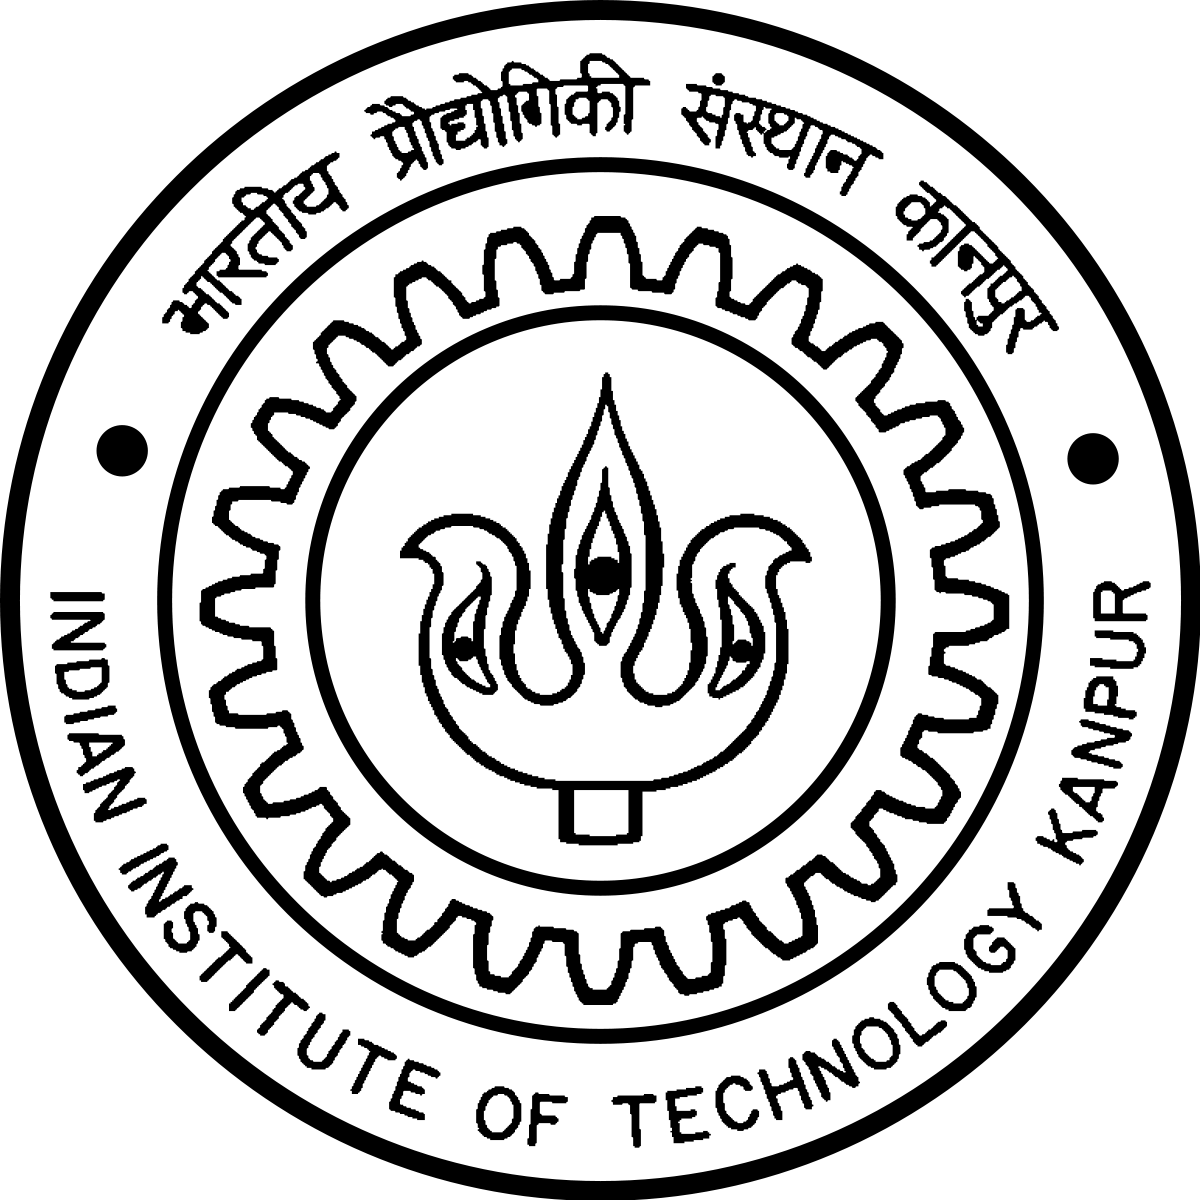
\includegraphics[width=0.3\textwidth]{images/iitk-logo.png}\\[15mm]
        \end{figure}
        \textsc{\LARGE Indian Institute of Technology Kanpur}\\[1cm]
        {\Large CS395A}\\[7mm]

        \hrule
        \vspace{3mm}
        \textbf{\Large Undergraduate Project - 1}\\[5mm]
        \hrule
        \vspace{3mm}

        \begin{multicols}{2}
            \textit{Students:}\\[2mm]
            Harish Rajagopal (160552)\\
            Vishwas Lathi (160808)\\

            \vfill\null\columnbreak

            \textit{Professor:}\\[2mm]
            Vinay Namboodiri\\
            Dept. of Computer Science and Engineering
        \end{multicols}
    \end{titlepage}

    \begin{center}
        \LARGE Project Report
        \vspace{15mm}
    \end{center}

    \begin{multicols}{2}
        \section{Abstract}
            We propose MAD-SRGAN which is a multi-agent generalisation to SRGAN \cite{srgan}.
            SRGAN, a generative adversarial network \cite{gan} for image super-resolution is capable of generating photo-realistic natural $4\times$ upscaled images.

            SRGAN consists of a single discriminator which tries to discriminate whether generated images are realistic or not, while the generator tries to push the generated image towards the manifold of natural images.
            MADGAN \cite{madgan} is a generalisation of GAN to address the problem of mode collapse, which most of the GAN's and their variants suffer.
            We propose a modification to vanilla SRGAN by combining MADGAN and SRGAN, namely MAD-SRGAN which consists of multiple generators and further variants also include multiple discriminators.

        \section{MAD-SRGAN}
            MAD-SRGAN consists of a 4 mini-generators each of which which deep residual network \cite{resnet} with skip connections, as shown in fig.~\ref{fig:gen-arch}.
            Each residual block consists of two convolution layers with $3\times3$ kernel and $64$ filters followed by batch-normalization \cite{batch-norm} layer and ReLU as the activation function.

            To discriminate whether the generated images lie close to natural images manifold, we have a discriminator network.
            The network uses the DCGAN \cite{dcgan} architecture.
            It consists of 8 convolution layers with $3\times3$ filter kernels.
            The feature maps obtained from the convolution layers are fed as input to two densely connected layers, which outputs the probability of classification using a sigmoid function.
            The network is trained using high-resolution images which are 4x downscaled and then fed as input to the model while the ground truth remains the upscaled images.

            \begin{figure}[H]
                \centering
                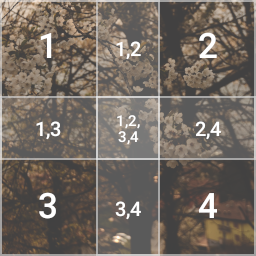
\includegraphics[width=0.25\textwidth]{images/overlap.png}
                \caption{Overlap in outputs}
                \label{fig:overlap}
            \end{figure}

            The input image is divided into four equal and slightly overlapping sections, each corresponding to the top-left, top-right, bottom-left and bottom-right portion of the input image (see fig.~\ref{fig:overlap}).
            Each section is then fed to a mini-generator which tries to generate the corresponding part in the high-resolution target image.
            The output of all the generators is concatenated in the same fashion as the division of the input image.
            This output is then passed as an input to the discriminator which tries to identify whether the input image is fake or not.

            Later on, in our experiments, we tried a multi-discriminator approach where the output of each mini-generator was fed to a mini-discriminator.
            The model consists of four mini-generators with sharing of parameters as defined earlier.
            Hence, the current model has four mini-discriminators, each trying to predict whether the section generated by the corresponding mini-generator, is fake or not.
            Then the outputs of all the mini-generators are combined in the same way as defined above and then given as input to a master discriminator which tries to compare the final upscaled image with the target and decides if it's real or not.

            \begin{figure*}
                \centering
                \begin{subfigure}{0.4\textwidth}
                    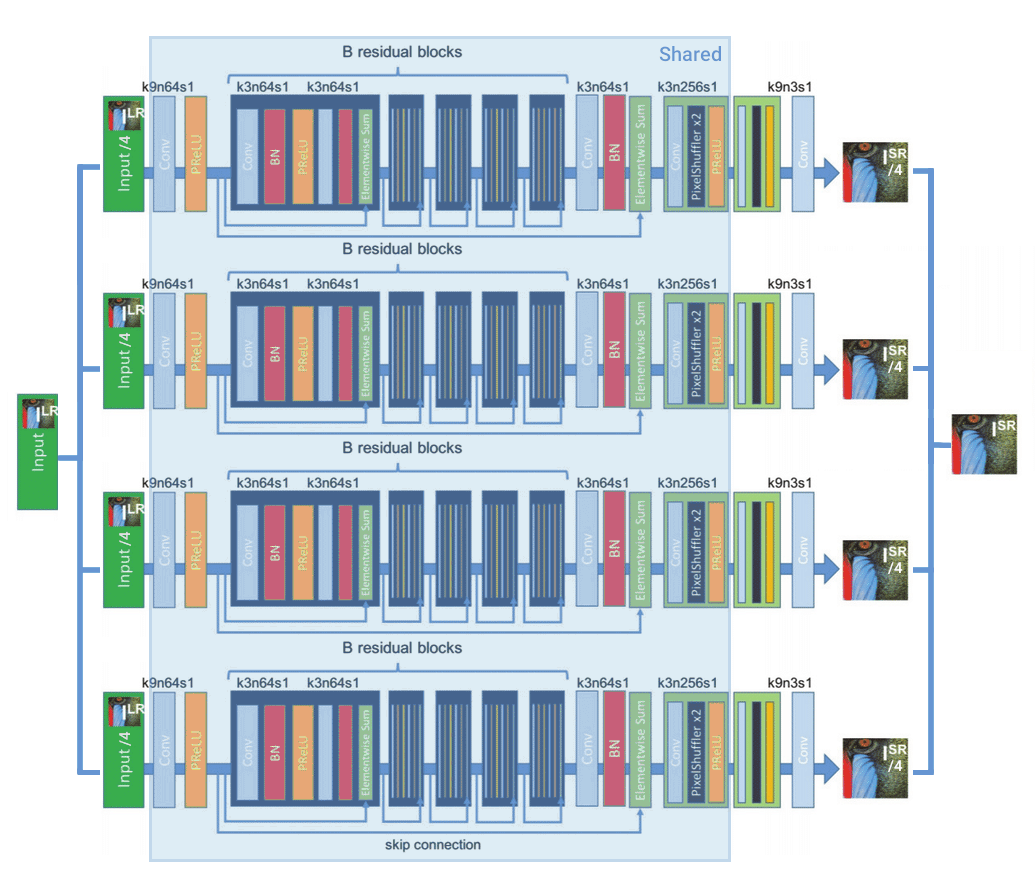
\includegraphics[width=\textwidth]{images/mad-srgan-gen-arch.png}
                    \caption{Generators}
                \end{subfigure}
                \begin{subfigure}{0.4\textwidth}
                    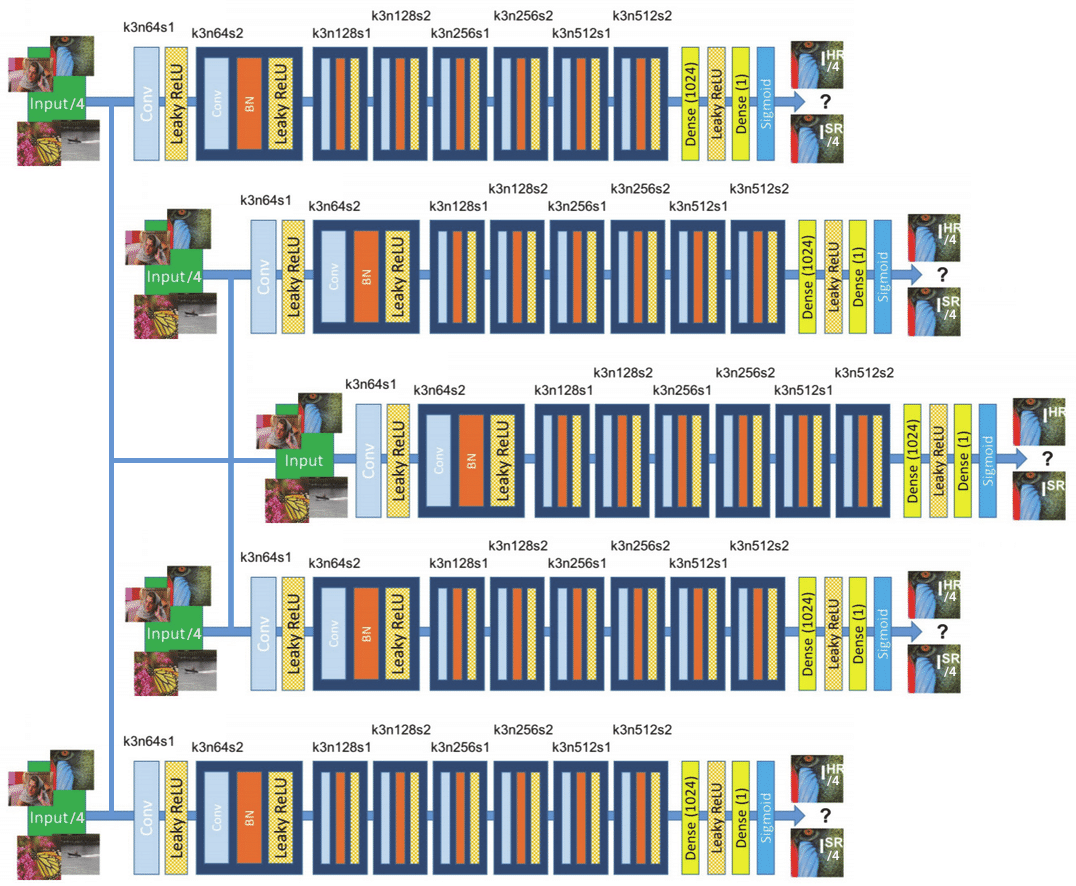
\includegraphics[width=\textwidth]{images/mad-srgan-disc-arch.png}
                    \caption{Discriminators}
                \end{subfigure}\\[3mm]
                \caption{MAD-SRGAN Architecture}
                \label{fig:gen-arch}
            \end{figure*}

        \section{Losses}
            The loss function $L$ consists of three parts, namely the content loss $(L_{content})$, adversarial loss $(L_{adv})$ and the overlap loss $(L_{overlap})$.
                $$L = L_{content} + \alpha L_{adv} + \beta L_{overlap}$$
            where $\alpha$ and $\beta$ are hyperparameters.

            The content loss is a perceptual loss \cite{perceptual} calculated on feature maps of the VGG19 network \cite{vgg}, similar to the one used by SRGAN.
            The adversarial loss is the adversarial loss for the generators by the discriminator, as used in SRGAN.
            The overlap loss is the MSE loss for the overlapping parts of the four generator outputs (see fig.~\ref{fig:overlap}), calculated as follows:
                $$L_{overlap} = \sum_{i=1}^3 \sum_{j=i+1}^4 MSE(i, j)$$
            where $MSE(i, j)$ is the MSE loss for the overlapping parts of images $i$ and $j$.

            In the multi-discriminator setup, the adversarial loss $L_{adv}$ now consists of adversarial loss corresponding to each multi-discriminator and the adversarial loss for the master-discriminator.
                $$L_{adv} = L_{adv}^{master} + \sum_{i=1}^{4}L_{adv}^{min\_disc\_i}$$

        \section{Experiments}
            \begin{figure*}
                \centering
                \begin{subfigure}{0.48\textwidth}
                    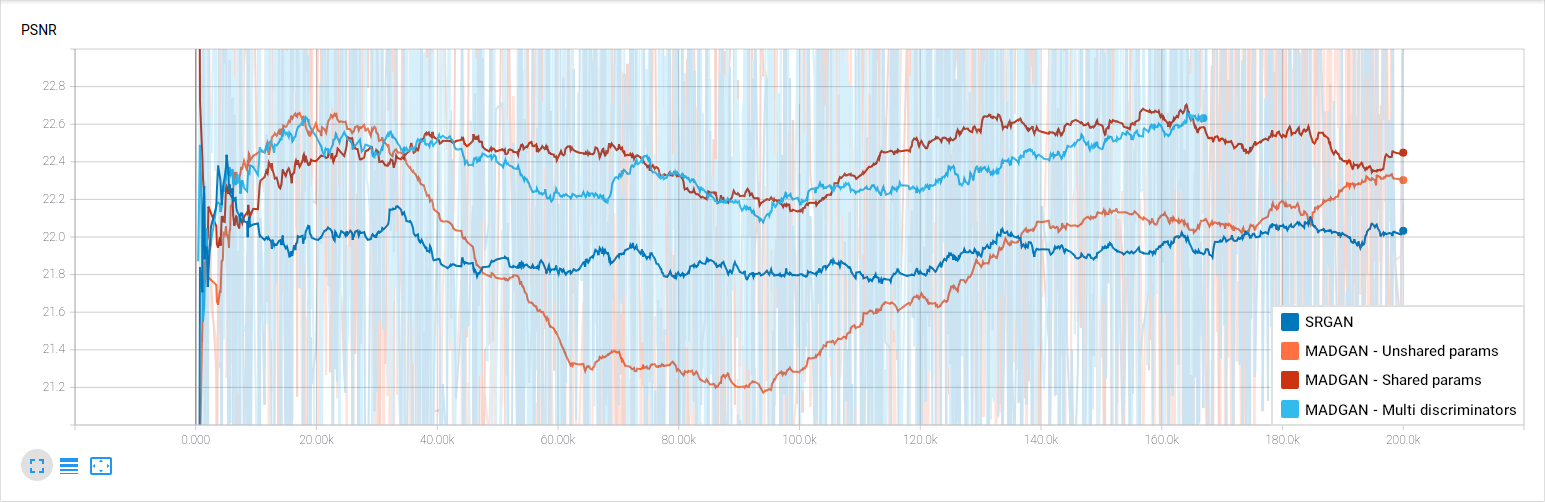
\includegraphics[width=\textwidth]{images/psnr.png}
                    \caption{PSNR}
                \end{subfigure}
                \quad
                \begin{subfigure}{0.48\textwidth}
                    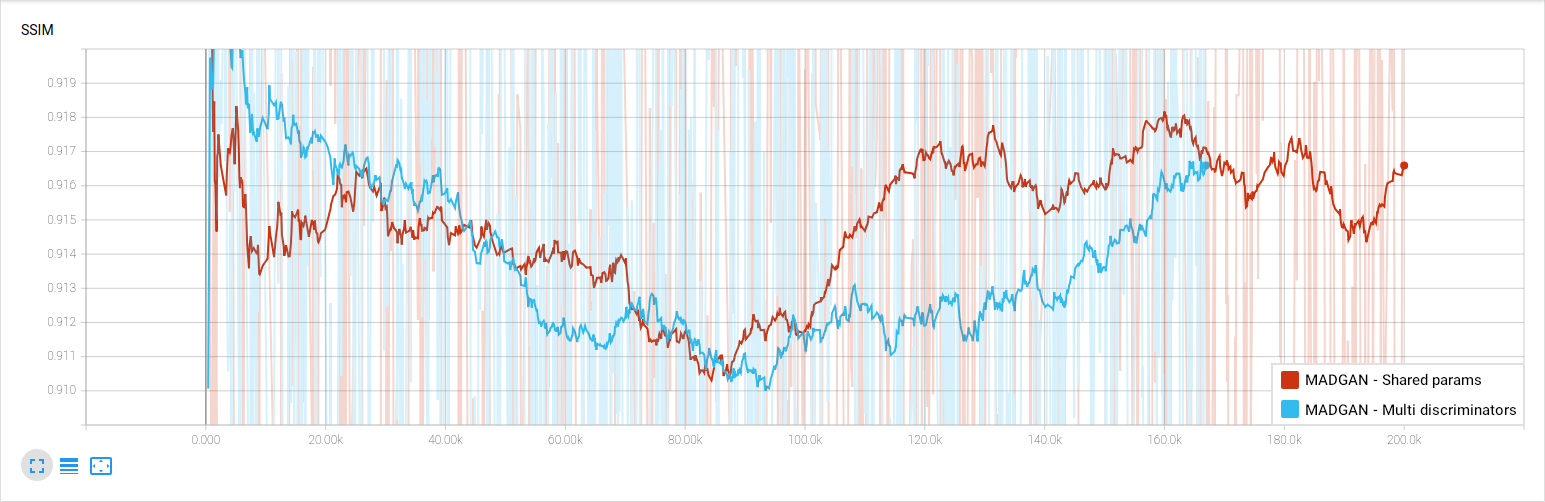
\includegraphics[width=\textwidth]{images/ssim.png}
                    \caption{SSIM}
                \end{subfigure}\\[5mm]
                \begin{subfigure}{0.48\textwidth}
                    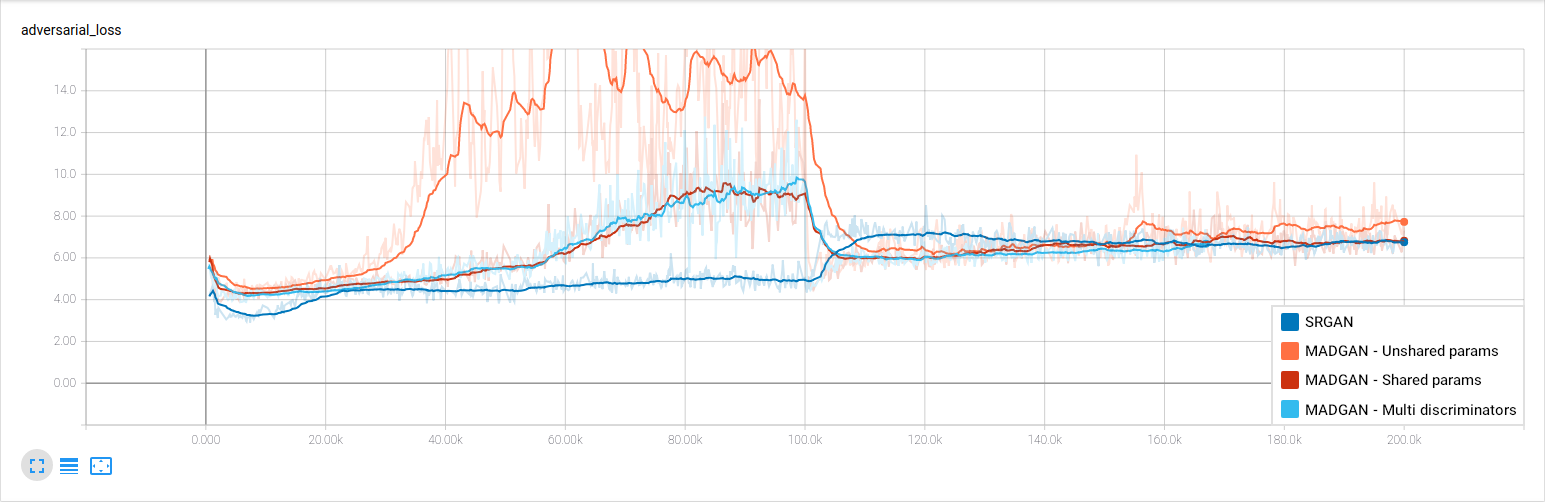
\includegraphics[width=\textwidth]{images/adv-loss.png}
                    \caption{Adversarial Loss}
                \end{subfigure}
                \quad
                \begin{subfigure}{0.48\textwidth}
                    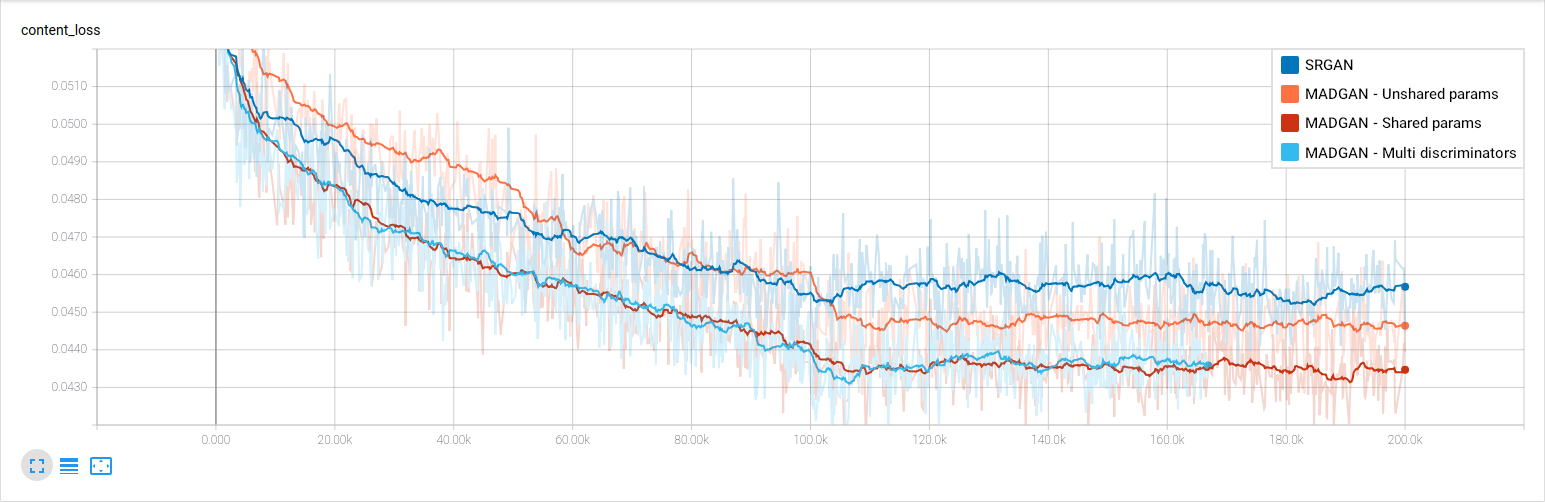
\includegraphics[width=\textwidth]{images/cont-loss.png}
                    \caption{Content Loss}
                \end{subfigure}\\[5mm]
                \begin{subfigure}{0.48\textwidth}
                    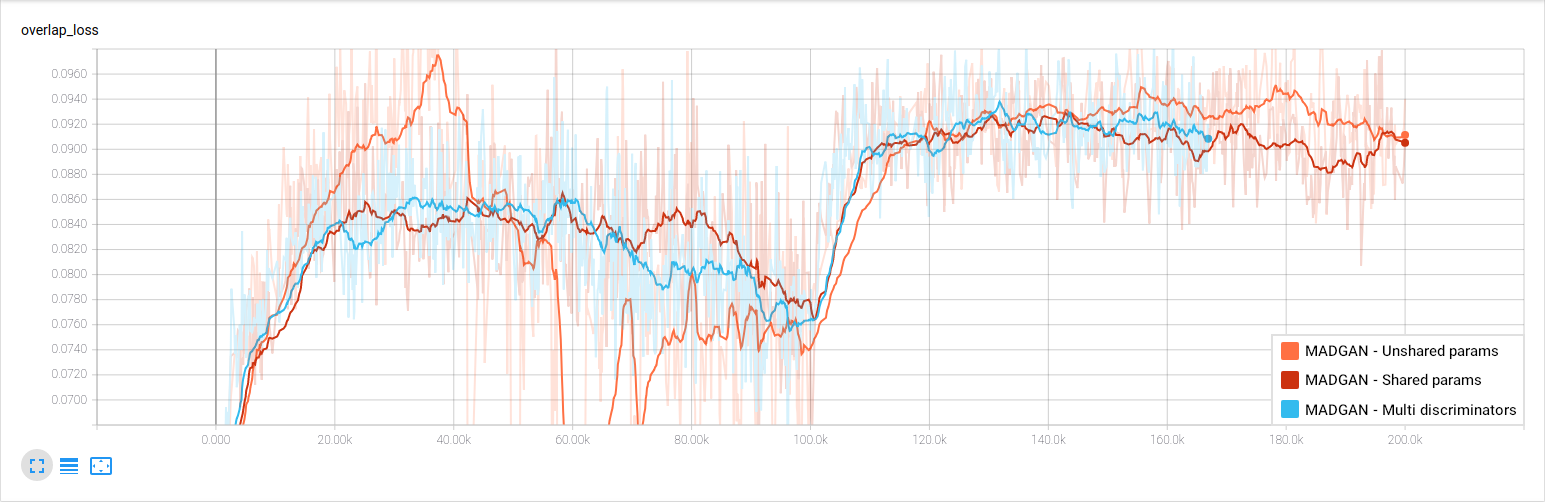
\includegraphics[width=\textwidth]{images/ovrl-loss.png}
                    \caption{Overlap Loss}
                \end{subfigure}\\[2mm]
                \caption{Results of MAD-SRGAN over SRGAN}
                \label{fig:results}
            \end{figure*}

            We ran our experiments using Tensorflow \cite{tensorflow} v1.10.
            The system setup was a GPU server running Ubuntu 14.04.5 LTS, with a 12-core Intel Core i7 CPU and a single Nvidia GeForce GTX TITAN X (12GB) graphics card.
            The code was adapted from the GitHub repository \href{https://github.com/brade31919/SRGAN-tensorflow}{SRGAN-tensorflow}, which is our reference SRGAN implementation.
            The model was trained on the RAISE dataset \cite{raise} and the TESTIMAGES dataset \cite{testimages-1,testimages-2} was used for testing on aliasing patterns.

            For image pre-processing, we applied random crop and random flipping to generate inputs of $24 \times 24$ pixels, with a 4x output.
            The optimiser used was Adam, with staircase decay for the learning rate.
            PSNR and multi-scale SSIM \cite{msssim} were the additional metrics used for evaluating.
            Additionally, we also used images applied in aliasing tests as test images, to gauge the performance of the model concerning possible aliasing effects.
            Sample image outputs along with outputs for aliasing test images are shown in the appendix on page \pageref{samples}.

            The values for our hyperparameters are:
            \begin{itemize}
                \item Batch size: 16
                \item Residual blocks: 16
                \item VGG scaling in perceptual loss: 0.0061
                \item Adversarial loss weight ($\alpha$): 0.001
                \item Overlap loss weight ($\beta$): 0.1
                \item Learning rate: 0.0001
                \item Learning rate decay rate: 0.1
                \item Learning rate decay after: 100000 steps
                \item Adam $\beta_1$ parameter: 0.9
                \item Maximum epochs: 200000
            \end{itemize}

            Results visualised via Tensorboard \cite{tensorflow} (see fig.~\ref{fig:results}) show that MAD-SRGAN with no sharing of parameters showed poor performance as compared to SRGAN, resulting in noisy images.
            Enabling sharing of parameters in the lower layers resulted in a noticeable improvement over keeping parameters separate, and slight improvements over SRGAN.
            We think that this is because sharing results in the lowering of model parameters and thus helps in the stabilization of training those parameters.
            Further, this would help focus the optimizer on fine-tuning the higher layers of the generators as per their requirements and not focus too much on getting the more basic processing required by the lower layers right.

            Addition of multiple discriminators in the form of one discriminator for each generator along with the global discriminator should help to tune the output of each generator further.
            However, we observed that this did not result in a noticeable improvement either in the losses, the metrics (PSNR or SSIM), or even when visually inspecting the output images.

        \bibliographystyle{ieeetr}
        \bibliography{refer}
    \end{multicols}

    \newpage

    \begin{center}
        \LARGE Appendix: Sample Images
    \end{center}\label{samples}

    \section*{Test Images}
        \begin{figure}[H]
            \centering
            \begin{subfigure}{0.2\textwidth}
                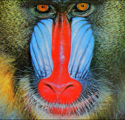
\includegraphics[width=\textwidth]{images/samples/img-1-input.png}
                \caption*{Input}
            \end{subfigure}
            \enspace
            \begin{subfigure}{0.2\textwidth}
                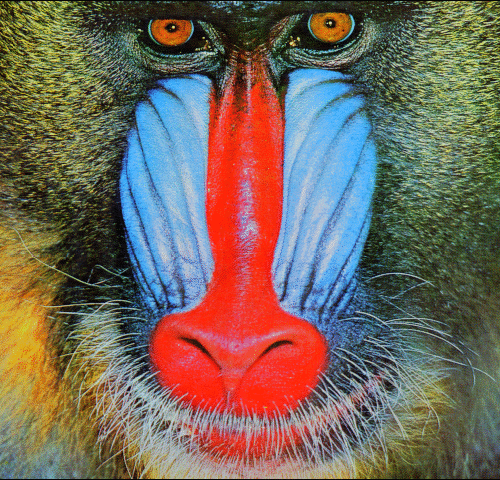
\includegraphics[width=\textwidth]{images/samples/img-1-orig.png}
                \caption*{Output}
            \end{subfigure}
            \enspace
            \begin{subfigure}{0.2\textwidth}
                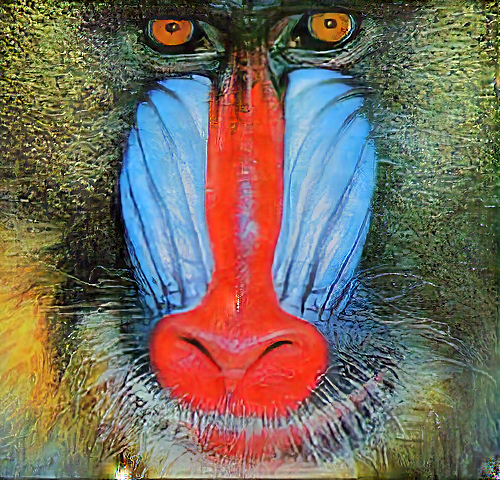
\includegraphics[width=\textwidth]{images/samples/img-1-srgan.png}
                \caption*{SRGAN}
            \end{subfigure}
            \enspace
            \begin{subfigure}{0.2\textwidth}
                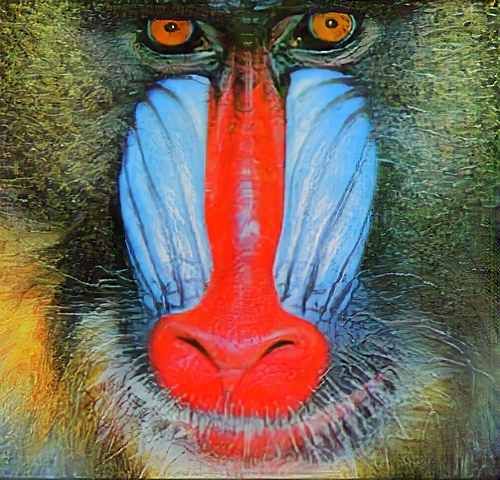
\includegraphics[width=\textwidth]{images/samples/img-1-mad-srgan.png}
                \caption*{MAD-SRGAN}
            \end{subfigure}
        \end{figure}

        \begin{figure}[H]
            \centering
            \begin{subfigure}{0.2\textwidth}
                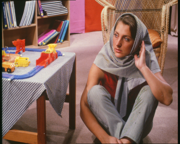
\includegraphics[width=\textwidth]{images/samples/img-2-input.png}
                \caption*{Input}
            \end{subfigure}
            \enspace
            \begin{subfigure}{0.2\textwidth}
                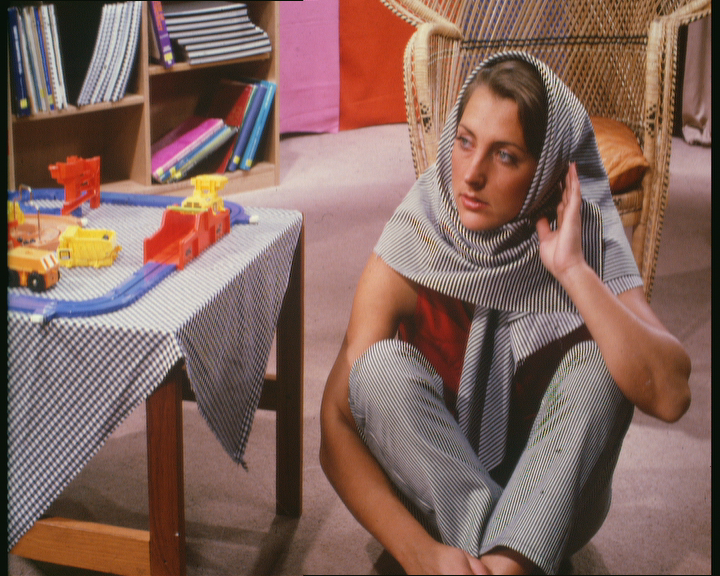
\includegraphics[width=\textwidth]{images/samples/img-2-orig.png}
                \caption*{Output}
            \end{subfigure}
            \enspace
            \begin{subfigure}{0.2\textwidth}
                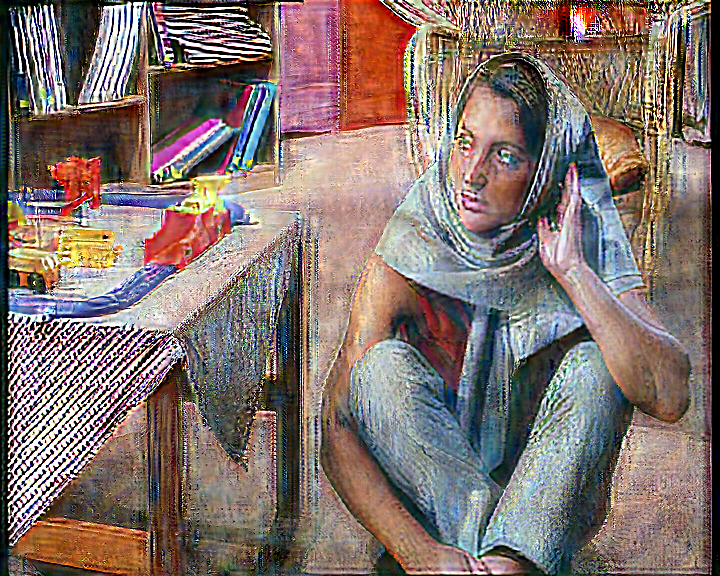
\includegraphics[width=\textwidth]{images/samples/img-2-srgan.png}
                \caption*{SRGAN}
            \end{subfigure}
            \enspace
            \begin{subfigure}{0.2\textwidth}
                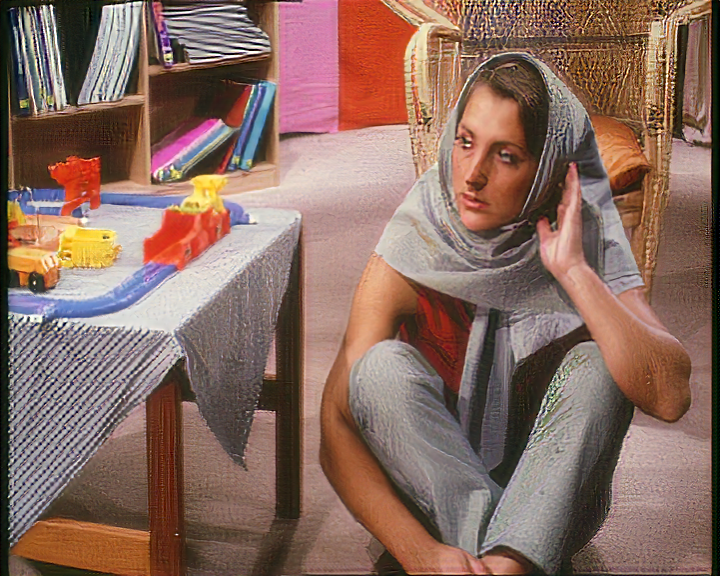
\includegraphics[width=\textwidth]{images/samples/img-2-mad-srgan.png}
                \caption*{MAD-SRGAN}
            \end{subfigure}
        \end{figure}

        \begin{figure}[H]
            \centering
            \begin{subfigure}{0.2\textwidth}
                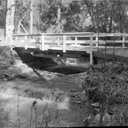
\includegraphics[width=\textwidth]{images/samples/img-3-input.png}
                \caption*{Input}
            \end{subfigure}
            \enspace
            \begin{subfigure}{0.2\textwidth}
                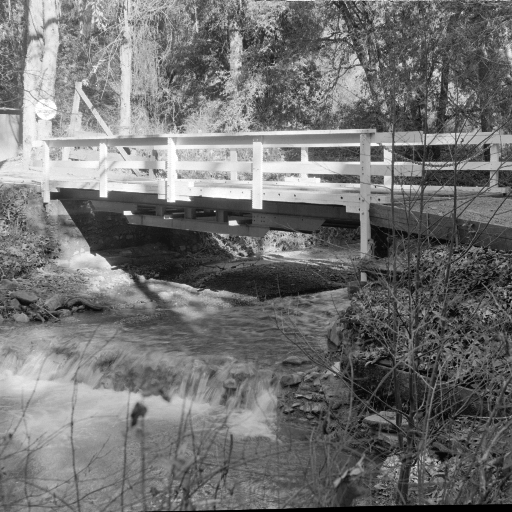
\includegraphics[width=\textwidth]{images/samples/img-3-orig.png}
                \caption*{Output}
            \end{subfigure}
            \enspace
            \begin{subfigure}{0.2\textwidth}
                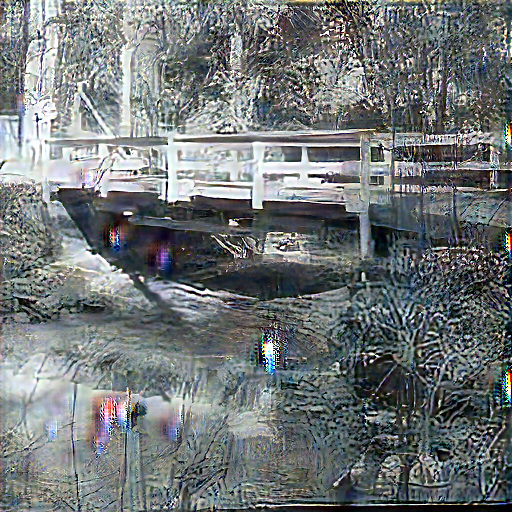
\includegraphics[width=\textwidth]{images/samples/img-3-srgan.png}
                \caption*{SRGAN}
            \end{subfigure}
            \enspace
            \begin{subfigure}{0.2\textwidth}
                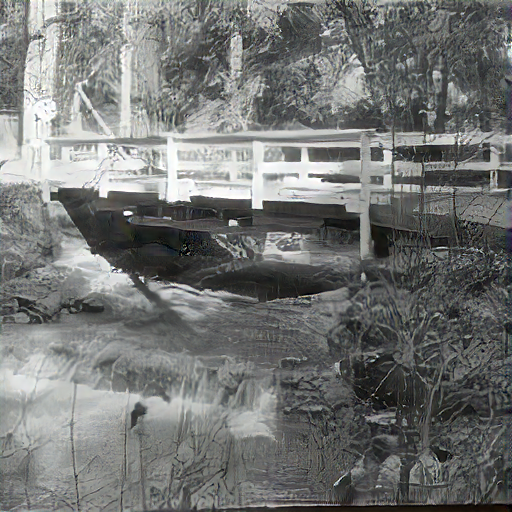
\includegraphics[width=\textwidth]{images/samples/img-3-mad-srgan.png}
                \caption*{MAD-SRGAN}
            \end{subfigure}
        \end{figure}

        \begin{figure}[H]
            \centering
            \begin{subfigure}{0.2\textwidth}
                
\includegraphics[width=\textwidth]{images/samples/img-4-input.png}
                \caption*{Input}
            \end{subfigure}
            \enspace
            \begin{subfigure}{0.2\textwidth}
                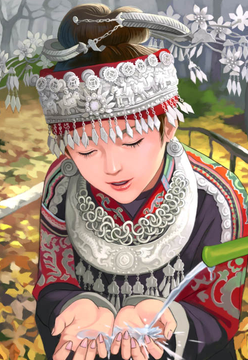
\includegraphics[width=\textwidth]{images/samples/img-4-orig.png}
                \caption*{Output}
            \end{subfigure}
            \enspace
            \begin{subfigure}{0.2\textwidth}
                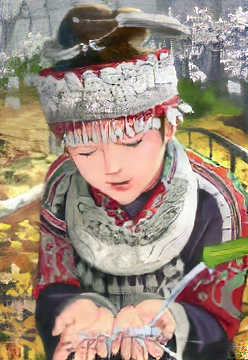
\includegraphics[width=\textwidth]{images/samples/img-4-srgan.png}
                \caption*{SRGAN}
            \end{subfigure}
            \enspace
            \begin{subfigure}{0.2\textwidth}
                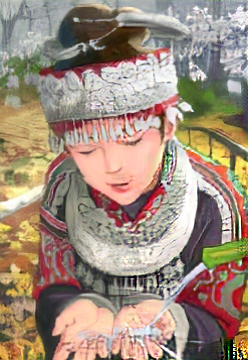
\includegraphics[width=\textwidth]{images/samples/img-4-mad-srgan.png}
                \caption*{MAD-SRGAN}
            \end{subfigure}
        \end{figure}

    \section*{Aliasing Patterns}
        \begin{figure}[H]
            \centering
            \begin{subfigure}{0.2\textwidth}
                
\includegraphics[width=\textwidth]{images/samples/aliasing-1-input.png}
                \caption*{Input}
            \end{subfigure}
            \enspace
            \begin{subfigure}{0.2\textwidth}
                
\includegraphics[width=\textwidth]{images/samples/aliasing-1-orig.png}
                \caption*{Output}
            \end{subfigure}
            \enspace
            \begin{subfigure}{0.2\textwidth}
                
\includegraphics[width=\textwidth]{images/samples/aliasing-1-srgan.png}
                \caption*{SRGAN}
            \end{subfigure}
            \enspace
            \begin{subfigure}{0.2\textwidth}
                
\includegraphics[width=\textwidth]{images/samples/aliasing-1-mad-srgan.png}
                \caption*{MAD-SRGAN}
            \end{subfigure}
        \end{figure}

        \begin{figure}[H]
            \centering
            \begin{subfigure}{0.2\textwidth}
                
\includegraphics[width=\textwidth]{images/samples/aliasing-2-input.png}
                \caption*{Input}
            \end{subfigure}
            \enspace
            \begin{subfigure}{0.2\textwidth}
                
\includegraphics[width=\textwidth]{images/samples/aliasing-2-orig.png}
                \caption*{Output}
            \end{subfigure}
            \enspace
            \begin{subfigure}{0.2\textwidth}
                
\includegraphics[width=\textwidth]{images/samples/aliasing-2-srgan.png}
                \caption*{SRGAN}
            \end{subfigure}
            \enspace
            \begin{subfigure}{0.2\textwidth}
                
\includegraphics[width=\textwidth]{images/samples/aliasing-2-mad-srgan.png}
                \caption*{MAD-SRGAN}
            \end{subfigure}
        \end{figure}

        \begin{figure}[H]
            \centering
            \begin{subfigure}{0.2\textwidth}
                
\includegraphics[width=\textwidth]{images/samples/aliasing-3-input.png}
                \caption*{Input}
            \end{subfigure}
            \enspace
            \begin{subfigure}{0.2\textwidth}
                
\includegraphics[width=\textwidth]{images/samples/aliasing-3-orig.png}
                \caption*{Output}
            \end{subfigure}
            \enspace
            \begin{subfigure}{0.2\textwidth}
                
\includegraphics[width=\textwidth]{images/samples/aliasing-3-srgan.png}
                \caption*{SRGAN}
            \end{subfigure}
            \enspace
            \begin{subfigure}{0.2\textwidth}
                
\includegraphics[width=\textwidth]{images/samples/aliasing-3-mad-srgan.png}
                \caption*{MAD-SRGAN}
            \end{subfigure}
        \end{figure}

        \begin{figure}[H]
            \centering
            \begin{subfigure}{0.2\textwidth}
                
\includegraphics[width=\textwidth]{images/samples/aliasing-4-input.png}
                \caption*{Input}
            \end{subfigure}
            \enspace
            \begin{subfigure}{0.2\textwidth}
                
\includegraphics[width=\textwidth]{images/samples/aliasing-4-orig.png}
                \caption*{Output}
            \end{subfigure}
            \enspace
            \begin{subfigure}{0.2\textwidth}
                \includegraphics[width=\textwidth]{images/samples/aliasing-4-srgan.png}
                \caption*{SRGAN}
            \end{subfigure}
            \enspace
            \begin{subfigure}{0.2\textwidth}
                \includegraphics[width=\textwidth]{images/samples/aliasing-4-mad-srgan.png}
                \caption*{MAD-SRGAN}
            \end{subfigure}
        \end{figure}
\end{document}
